%%%%%%%%%%%%%%%%%%%%%%%%%%%%%%%%%%%%%%%%%%%%%%%%%%%%%%%%%%%%%%
%%%%		PLANTILLA LATEX PARA INFORMES
%%%%			LATEX REPORT TEMPLATE
%%%%	
%%%%	Autor	: Carlos Gonzalez Cortes
%%%%	Correo	: carlgonz@ug.uchile.cl
%%%%	Version	: 1.0
%%%%
%%%%	Notas	: Este codigo se entrega tal cual es y sin
%%%%			  ningun tipo de garantia. Sientase libre de
%%%%			  modificar y compartir.(acentos omitidos en
%%%%			  los comentarios por compatibilidad)
%%%%
%%%%%%%%%%%%%%%%%%%%%%%%%%%%%%%%%%%%%%%%%%%%%%%%%%%%%%%%%%%%%%




\documentclass[11pt,letterpaper]{article}
\usepackage[spanish]{babel}
\usepackage[table]{xcolor}
%\usepackage[ansinew]{inputenc}
\usepackage[utf8]{inputenc}
% \usepackage[latin1]{inputenc}
\usepackage[letterpaper,includeheadfoot, top=0.5cm, bottom=3.0cm, right=2.0cm, left=2.0cm]{geometry}
\renewcommand{\familydefault}{\sfdefault}

\usepackage{graphicx}
\usepackage{color}
\usepackage{hyperref}
\usepackage{amssymb}
\usepackage{url}
%\usepackage{pdfpages}
\usepackage{fancyhdr}
\usepackage{hyperref}
\usepackage{subfig}

\usepackage{listings} %Codigo
\lstset{language=C, tabsize=4,framexleftmargin=5mm,breaklines=true}

\begin{document}
%\begin{sf}
% --------------- ---------PORTADA --------------------------------------------
\newpage
\pagestyle{fancy}
\fancyhf{}
%-------------------- CABECERA ---------------------
\fancyhead[L]{ 
\includegraphics[scale=0.9]{img/logo.pdf} }
%------------------ TÍTULO -----------------------
\vspace*{6cm}
\begin{center}
\Huge  {Tarea 3 - Skip Lists, ABBs y ABBs Aleatorizados}\\
\vspace{1cm}
%\vspace{1cm}
%\small {Título pe} \\
\end{center}
%----------------- NOMBRES ------------------------
\vfill
\begin{flushright}
\begin{tabular}{ll}
Alumnos: & Jonathan Urzúa\\
		& José Manuel Aguilera\\
Profesor: & Gonzalo Navarro\\
& \today\\
& Santiago, Chile.
\end{tabular}
\end{flushright}

% ·············· ENCABEZADO - PIE DE PAGINA ············
\newpage
\pagestyle{fancy}
\fancyhf{}

%Encabezado
%\fancyhead[L]{\rightmark}
\fancyhead[L]{\small \rm \textit{Sección \rightmark}} %Izquierda
\fancyhead[R]{\small \rm \textbf{\thepage}} %Derecha


%\fancyfoot[L]{\small \rm \textit{Pie de página - Izquierda}} %Izquierda
%\fancyfoot[R]{\small \rm \textit{Pie de página - Derecha}} %Derecha
%\fancyfoot[C]{\thepage} %Centro

\renewcommand{\sectionmark}[1]{\markright{\thesection.\ #1}}
\renewcommand{\headrulewidth}{0.5pt}
\renewcommand{\footrulewidth}{0.5pt}

% =============== INDICE ===============

\tableofcontents
\listoffigures

% =============== SECCION ===============
\newpage
\section{Resumen}

Existen muchos tipos de estructuras de datos, dentro de las cuales están los Árboles de Búsqueda Binaria, los Árboles de Búsqueda Binaria Aleatorizados y las Skip Lists.\\

Los árboles de búsqueda binaria son estructuras de nodos, donde cada nodo puede tener solo dos hijos, el valor almacenado en el hijo izquierdo es siempre menor que el valor almacenado en el padre, y el valor almacenado en el hijo derecho es siempre mayor al valor almacenado en el padre. Esto genera un orden que permite realizar operaciones más eficientes sobre los datos.\\

Las Skip List son listas enlazadas, que utilizando otras listas auxiliares paralelas, permiten realizar saltos o atajos por sobre la lista principal, agilizando el movimiento sobre la estructura, y por lo tanto la eficiencia de las operaciones.\\

Este trabajo presenta las estructuras mencionadas, las explica y las analiza, para luego concluir sobre el comportamiento de sus operaciones, además de sus tiempos.\\

Finalmente, se logró llegar a la conclusión de que dado las condiciones de los experimentos presentaban una entrada de datos correspondiente a secuencias ordenadas, se presentó el peor caso para los ABB y estos se comportaron como $O(n)$. La altura de las Skip List presentó $O(\log(n))$, y su eficiencia en las operaciones fue también desfavorable debido a la forma del input, comportandose de manera similar a los ABB.

\newpage
\section{Introducción}

Las estructuras de datos son formas de organizar conjuntos de datos con el objetivo de facilitar su manipulación. Estas definen la organización de los datos y diferentes operaciones posibles para realizar sobre ellos.\\
Las operaciones más comunes que implementan las estructuras de datos son: Inserción, Eliminación y Búsqueda. Como sus nombres lo indican, Inserción se encarga de introducir un nuevo elemento a la estructura, Eliminación borra cierto elemento de la estructura y Búsqueda permite encontrar un elemento dentro de esta.\\

Dentro de las estructuras de datos más comunes y útiles están los Árboles de Búsqueda Binaria, o ABB. Estos árboles están definidos de forma recursiva y almacenan los elementos ordenados de izquierda a derecha, de menor a mayor (o al revés, dependiendo de la implementación). En otras palabras, dado un subarbol, la raíz de este es siempre mayor (o menor) a todos los elementos de su subarbol izquierdo, y es siempre menor (o mayor) a todos los elementos de su subarbol derecho.\\

Los ABB tienen muchas variantes, dentro de estas existe el Árbol de Búsqueda Binaria Aleatorizado, o Randomized Binary Tree en inglés. Estos corresponden a ABBs con ciertas componentes aleatorias en sus operaciones. En la Inserción, se considera que cada elemento tiene la probabilidad $1/n$ de ser la raíz del árbol, con $n$ el número de elementos en el árbol.\\

Existen otros tipos de estructuras para almacenar elementos ordenados. Uno de estos son las llamadas Skip Lists, que permiten almacenar objetos en listas enlazadas ordenadas. La idea principal es utilizar listas enlazadas paralelas, generando una especie de capas, donde la capa de más abajo constituye una lista enlazada con todos los elementos, y las capas superiores funcionan como una vía para saltar elementos de forma más rápida con respecto a su capa inferior.\\

Este trabajo se enfoca principalmente en el estudio de estas tres estructuras, experimentando con distintos volúmenes de datos y comparando la eficiencia de sus operaciones.

\newpage
\section{Análisis del problema}

La utilidad de las estructuras de datos para resolver problemas computacionales es significativo, tanto para mejorar la eficiencia del manejo de grandes cantidades de datos como para facilitar el uso de estos. Este trabajo se enfocará principalmente en el análisis de tres estructuras de datos: Skip Lists, Árboles de Búsqueda Binarios y Árboles de Búsqueda Binarios Aleatorizados.\\

Un árbol binario es una estructura de datos compuesta por nodos que pueden contener información y tienen un hijo izquierdo y un hijo derecho. Cada nodo puede tener solo dos hijos.\\
El árbol de búsqueda binaria es un árbol binario en el que sus nodos tienen un orden particular y se definen de la siguiente manera:\\

Un árbol binario no vacío, de raíz $R$, se define recursivamente de la siguiente manera:
\begin{itemize}
\item Si $R$ tiene un subárbol izquierdo, $R$ es mayor que el valor máximo presente en el subárbol izquierdo, y este es un ABB.
\item Si $R$ tiene un subárbol derecho, $R$ es menor que el valor mínimo presente en el subárbol derecho, y este es un ABB.
\end{itemize}

Esta definición es para un ABB con orden creciente, pero es perfectamente válido un ABB decreciente, por lo que es relativo a la implementación y las necesidades para las cuales se utiliza la estructura.
	
\begin{figure}[htb]
	\centerline{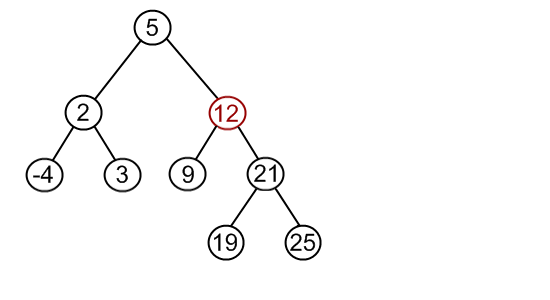
\includegraphics[scale=0.6]{img/bst.png}}
	\caption{ABB} \label{bst}
\end{figure}

La inserción y la búsqueda se basan en la propiedad de orden que tiene la estructura.

Dado un elemento $x$ que se quiere buscar en el árbol $R$, la búsqueda es de la siguiente forma:
\begin{itemize}
\item Se compara $x$ con el elemento en la raíz de $R$. Si son iguales, retornar el elemento.
\item Si $x$ es menor al elemento en la raíz de $R$, repetir el procedimiento con la raíz del subárbol izquierdo de $R$. Si es mayor, repetir el procedimiento con la raíz del subárbol derecho de $R$.
\item Si se está en una hoja, y los elementos no son iguales, el elemento no se encuentra en el árbol.
\end{itemize}

Dado un elemento $x$ que se quiere insertar en el árbol $R$, la inserción es de la siguiente forma:
\begin{itemize}
\item Si la raíz de $R$ es vacía, insertar $x$ en el nodo.
\item Si $x$ es menor que el valor del nodo, y este no tiene hijo izquierdo, insertar $x$ como hijo izquierdo.
\item Si $x$ es mayor que el valor del nodo, y este no tiene hijo derecho, insertar $x$ como hijo derecho.
\item Si $x$ es menor que el valor del nodo, y tiene hijo izquierdo, repetir el procedimiento en el subárbol izquierdo del nodo.
\item Si $x$ es mayor que el valor del nodo, y tiene hijo derecho, repetir el procedimiento en el subárbol derecho del nodo.
\end{itemize}

El ABB asegura un promedio en el tiempo de inserción y búsqueda de $O(\log(n))$. Sin embargo, en el peor caso, el árbol podría quedar muy mal balanceado y obtener una altura de $O(n)$.

\newpage

El ABB Aleatorizado introduce modificaciones a las operaciones. La idea es agregar una componente de aleatoriedad. La inserción, en particular, ahora considera que cada elemento tiene $1/n$ probabilidad de ser raíz del árbol, con $n$ el número de elementos en el árbol.\\

La operación de inserción aleatorizada tendría entonces la siguiente forma (en pseudo-código):

\begin{figure}[htb]
	\centerline{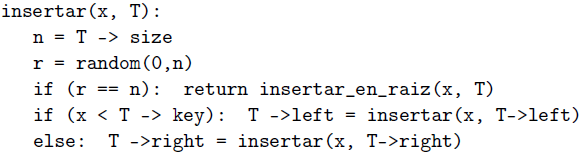
\includegraphics[scale=0.6]{img/insertar.png}}
	\caption{Inserción en ABB Aleatorizado} \label{insercionrandom}
\end{figure}

La aleatorización de un ABB tiene como finalidad reducir los casos en los cuales se forma un ABB muy poco balanceado (llegando a parecer casi listas enlazadas) y así poder asegurar mejor un comportamiento $O(\log(n))$.\\

La Skip List, por otro lado, corresponde a un tipo de estructura de datos distinto, relacionado con las listas enlazadas. Se compone por varias listas enlazadas paralelas, en forma de capas. La lista principal, que apunta a los datos reales, es una lista enlazada simple. Por sobre esta lista se construyen otras para formar una especie de atajo o vía rápida a los datos en la lista principal. Cada lista auxiliar funciona como un atajo para la que está por debajo.\\

Al igual que los ABB, la Skip List asegura un tiempo promedio de búsqueda de $O(\log(n))$.

\begin{figure}[htb]
	\centerline{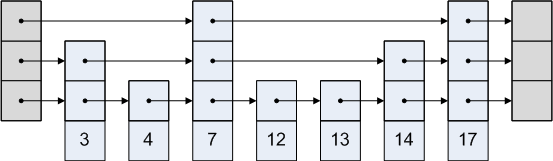
\includegraphics[scale=0.6]{img/skiplist.png}}
	\caption{Skip List} \label{skiplist}
\end{figure}

\newpage
\section{Solución del problema}

Con el fin de comparar las tres estructuras de datos que se han presentado en las secciones anteriores, se implementaron estas en Python, con el fin de poder experimentar y analizar sus comportamientos y tiempos con respecto a dos operaciones relevantes: Inserción y Búsqueda.

Los puntos relevantes para efectuar dicha comparación son los siguientes:
\begin{itemize}
\item Medir experimentalmente los tiempos de inserción y búsqueda mediante el número de comparaciones de llaves que se efectuan en cada operación.
\item Calcular alturas promedio de los árboles.
\end{itemize}

Para asegurar que las pruebas a las cuales se someterán las estructuras son concluyentes, se tomarán las siguientes consideraciones:
\begin{itemize}
\item Se generarán secuencias ordenadas de $n$ números, con $n \in \{ 10^4, 2\times10^4, 5\times10^5 \}$.
\item Los números generados corresponderán al intervalo de enteros $[ 0. 10^5 ]$.
\end{itemize}

Se insertarán las secuencias de números generados en las estructuras, para luego proceder a buscar $m$ valores en ellas, donde $m = 0.5 \times n$. Dentro de las búsquedas, se forzará que un $25\%$ de ellas sean infructuosas.\\

Con el procedimiento anterior se espera poder obtener información relevante del comportamiento de las estructuras, y poder concluir si realmente se comportan dentro de lo esperado. Por otro lado, se quiere visualizar el rendimiento de las estructuras en comparación.

\newpage
\section{Resultados}

Se implementó un set de tests en Python con el fin de llevar a cabo los experimentos propuestos en la sección anterior. Estos experimentos se corrieron 14 veces bajo cada uno de los criterios mencionados, para así asegurar un comportamiento promedio sobre las estructuras.\\

\textbf{ABBs:}\\

Búsqueda:

\begin{center}
    \begin{tabular}{| l | l | l |}
    \hline
    \textbf{Número de elementos} & \textbf{Número de comparaciones promedio} & \textbf{Tiempo promedio} \\
    \hline
    10000 & - & -\\
    \hline
    20000 & - & -\\
    \hline
    50000 & - & -\\
    \hline
    \end{tabular}
\end{center}

Inserción:

\begin{center}
    \begin{tabular}{| l | l | l |}
    \hline
    \textbf{Número de elementos} & \textbf{Número de comparaciones promedio} & \textbf{Tiempo promedio} \\
    \hline
    10000 & 49995000.0 & 23.53\\
    \hline
    20000 & 199990000.0 & 95.78\\
    \hline
    50000 & 1249975000.0 & 623.73\\
    \hline
    \end{tabular}
\end{center}

\textbf{Skip Lists:}\\

Búsqueda:

\begin{center}
    \begin{tabular}{| l | l | l | l |}
    \hline
    \textbf{Número de elementos} & \textbf{Número de comparaciones promedio} & \textbf{Altura promedio} & \textbf{Tiempo promedio} \\
    \hline
    10000 & 263667.28 & 14.85 & 0.09 \\
    \hline
    20000 & 643668.0 & 16.35 & 0.22 \\
    \hline
    50000 & 1595420.35 & 16.35 & 0.53 \\
    \hline
    \end{tabular}
\end{center}

Inserción:

\begin{center}
    \begin{tabular}{| l | l | l | l |}
    \hline
    \textbf{Número de elementos} & \textbf{Número de comparaciones promedio} & \textbf{Altura promedio} & \textbf{Tiempo promedio} \\
    \hline
    10000 & 129697.35 & 14.35 & 0.16 \\
    \hline
    20000 & 280626.42 & 16.21 & 0.34 \\
    \hline
    50000 & 780344.21 & 16.92 & 1.03 \\
    \hline
    \end{tabular}
\end{center}

\newpage
\section{Conclusiones}

Debido a que la entrada inicial para los ABB debía ser una secuencia ordenada de números, estos presentaron un comportamiento poco favorable dado que se presentó el peor caso posible. Este comportamiento es de $O(n)$. Se propone que con el fin de que los ABB se comporten de manera más favorable y eficiente, el input debe estar desordenado razonablemente.\\

Por otro lado, las Skip List presentaron un comportamiento $O(\log(n))$ con respecto a sus alturas, como era lo esperado. Su comportamiento a nivel de eficiencia no fue tan favorable debido a la forma del input inicial y presentó una forma similar a los ABBs.\\
Dentro del tiempo que tomaron las pruebas de inserción y búsqueda en las Skip List, es posible notar coherencia entre ambas operaciones viendo el tiempo promedio requerido para las pruebas, que crece a un ritmo similar.\\

\textbf{Comentario extra del equipo:} Debido a un error simple de código en la test suite que se creó para este trabajo, se terminó corriendo una cantidad muy grande de tests donde los datos de la búsqueda en ABB no se registraron. No es nuestra política inventar datos y por esta razón en las tareas anteriores hemos adjuntado los resultados que se generan en las test suites que creamos. Al ver el código de la implementación es fácil ver que debería haberse registrado como corresponde, al igual que las otras operaciones en las otras estructuras.

% ============= FIN DE DOCUMENTO ==============
\end{document}